\chapter{Cluster Analysis} \label{sec:clusteranalysis}
Cluster analysis is a task that groups objects from the input set so that each group consists of objects with similar properties. Similar means that same property of two objects differs minimally in comparison to same property of other nearest objects or all objects in cluster. This means that each cluster contains objects that are more similar to nearest neighbors or all objects from cluster than objects from other clusters. Hence the cluster analysis may be performed only on sets of objects which must be to each other comparable. This analysis has a wide range of applications, such as data mining, pattern recognition, machine learning, and many more.\\
Cluster analysis itself is only a task to be solved, not a concrete algorithm. There are many ways to solve this task, but they differ significantly in defining what cluster is and in cluster search efficiency. Most common definitions of the cluster are groups with small distances between the objects from the same cluster, dense areas of the input data, intervals or each particular statistical distribution.\\
For mathematical definition of the problem, we will take a real vector as an object where each dimension presents an object property. If we consider objects as a set of vectors $M$, distance will be a function $d:M\times M \to \mathbb{R}$ fulfilling metric axioms:\\ \\
$ \forall  a,b,c \in M$
\begin{enumerate}
\item $d(a,b)\geq 0$ \textit{(non-negativity)}
\item $d(a,b) = 0 \iff a = b$ \textit{(identity)}
\item $d(a,b) = d(b,a)$ \textit{(symmetry)}
\item$d(a,b) \leq d(a,c) + d(c,b)$ \textit{(triangle inequality)}
\end{enumerate}

\section{Cluster organization} \label{sec:clusterorganization}
Object organization into clusters could be done several ways depends on structure of clusters and number of clusters into which an object belongs.
\begin{description}
\item[Hard clustering] is clustering, where each object belongs to one and only one cluster. This means that hard clustering creates system where clusters are disjoint sets.
\item[Fuzzy clustering] assigns objects to clusters too, but difference is that object can belong to more than one cluster. The object membership to cluster could be specified by strength of this membership so object could belongs to cluster more or less based on similarity.
\item[Hierarchical clustering] is hierarchically ordered clusters creates which creates a system of subsets where the intersection of the two is either the empty set or just one of them so clusters creates structures like n-ary trees. Because of complexity of the hierarchical clustering, in this thesis we deal with non-hierarchical type only.
\end{description}

There are many cluster models but in next section~\ref{sec:clustermodels}, only the best known will be described. One of the reasons why there exists a large amount of them is that the ``cluster'' cannot be precisely defined~\cite{EstivillCastro02}. Second reason is really wide applicability of this task so people from different departments approach this problem differently, because their notion of cluster differs significantly. \\

\section{Cluster Models and Algorithms} \label{sec:clustermodels}
There exist many clustering algorithms because of many cluster models. Problem is that there exist no universal algorithm, such an algorithm that covers all cluster models. Each algorithm was designed to cover one model or a subset of models and usually it is weak or not applicable for other models.
\subsection{Distances}
Because all of these algorithms counts distance, appropriate metric must be used.
\begin{description}
\item[Manhattan distance $L_1$] $$\|a-b\|_1=\sum_i |a_i - b_i| $$
\item[Euclidian distance $L_2$] $$\|a-b\|_2=\sqrt{\sum_i (a_i - b_i)^2 }$$
\item[Squared Euclidian distance $L_2^2$] $$\|a-b\|_2^2=\sum_i (a_i - b_i)^2 $$
\item[$p$-norm distance $L_p$] $$\|a-b\|_p=\Big(\sum_i |a_i - b_i|^p\Big)^\frac{1}{p} $$
\item[Maximum distance $L_\infty$] $$\|a-b\|_\infty=\lim_{p\to\infty}\Big(\sum_i |a_i - b_i|^p\Big)^\frac{1}{p}=\max_i |a_i - b_i| $$
\end{description}
All of these distances are $L_p$ distances and they are applicable on $\mathbb{R^d}$ spaces only. For other types, different metrics must be used.\\

We could also tak distance functions usable in statistics like \textbf{Mahalanobis distance} and \textbf{Wasserstein metric}

\subsubsection{Mahalanobis distance}
Is useful if we need to compute distances between a point $P$ and distribution $D$. The main idea of this distance is measuring ho differs $P$ from the mean of $D$.
If we have observation $p=(p_1,...,p_n)^T$ a mean of set of observations $\mu=(\mu_1,...,\mu_n)^T$ and a covariance matrix $S$, the Mahalanobis distance is defined as:
$$D_M(x) = \sqrt{(x - \mu)^T S^{-1} (x-\mu)}$$

\subsubsection{Wasserstein metric}
Another distance used in statistics is Wasserstein metric (also called Earth mover's distance (EMD))~\cite{Vallender73}. This metric is used for compute distance between two probability distributions on given metric space $M$. There is analogy with moving ``dirt'' piled up in same way as shape of probability distribution. The distance is amount of ``dust'' which must be moved to change the shape of pile into another shape specified by second probability distribution times the distance it has to be moved. This distance is defined by following way:\\
Let $X$ be a metric space with metrix $\rho$ and $\mathfrak{B}$ be the $\sigma$-algebra of Borel subsets of $X$. The Wasserstein distance $R(P,Q)$ between probability distributions $P$ and $Q$ on $(X, \mathfrak{B})$ is defined as:
$$R(P,Q)=\inf\mathbf{E}\rho(\xi, \sigma)$$
where $\inf$ is taken over all possible pairs of random variables $\xi$ and $\sigma$ with distribution $P$ and $Q$.\\

There are also spaces, which are even not from mathematics but which contains objects that are also comparable.

\subsubsection{Levenshtein distance} Levenshtein distance is used for edit distance between two strings $a, b$ and it is recursively defined by following definition:
\begin{equation*}
lev_{a,b}(i,j)=
\begin{cases}
max(i,j) & $if $ min(i,j)=0, \cr
min \begin{cases}
lev_{a,b}(i-1,j) + 1 \cr
lev_{a,b}(i,j-1) + 1 \cr
lev_{a,b}(i-1,j-1) + dif(a_i,b_j)
\end{cases} & $otherwise$
\end{cases}
\end{equation*}
Where \begin{equation*}
dif(a_i,b_j)=
\begin{cases}
0 & $if $ a_i = b_j, \cr
1 & $otherwise$
min 
\end{cases}
\end{equation*}

\subsubsection{Signature Quadratic Form Distance}
This metric becomes really useful for comparing multimedia objects, which could be described by signatures. Problem is that these signatures could differ in structure and size so we could not use distances described before. The feature of each object is described by a vector of pairs of centroid from feature space $\mathbb{FS}$ and its weight from $\mathbb{R^{+}}$.
Than we do not count distances between the feature signatures but in Signature Quadratic Form Distance~\cite{Beecks10}, the similarity functions are used.
Mathematically, Signature Quadratic Form Distance (SQFD) is defined for two feature signatures $S^{q} = \{\{c_i^q, w_i^q\}|i=1,...,n\}$ and $S^{o} = \{\{c_i^o, w_i^o\}|i=1,...,m\}$ and a similarity function $f_s(c_i,c_j) \to \mathbb{R}$ as:
$$SQFD_{f_s}(S^q,S^o)=\sqrt{(w_q|-w_o)A_{f_n}(w_q|-w_o)^T}$$
where $A_{f_n} \in \mathbb{R}^{(n+m)\times(n+m)}$ is the similarity matrix generated by applying similarity function $f_s$ to the corresponding centroids ($a_{ij}-f_s(c_i,c_j)$) and operator $|$ means concatenation of two vectors, so $w_q|-w_o = (w_1^q,...,w_n^q,-w_1^o,...,-w_m^o)$


\subsection{Cluster models}
Because definitions of cluster differs, there are also many definition of cluster models. In following section, the most known models will be described.

\begin{figure}[h]
\centering
\begin{subfigure}{.49\textwidth}
  \centering
  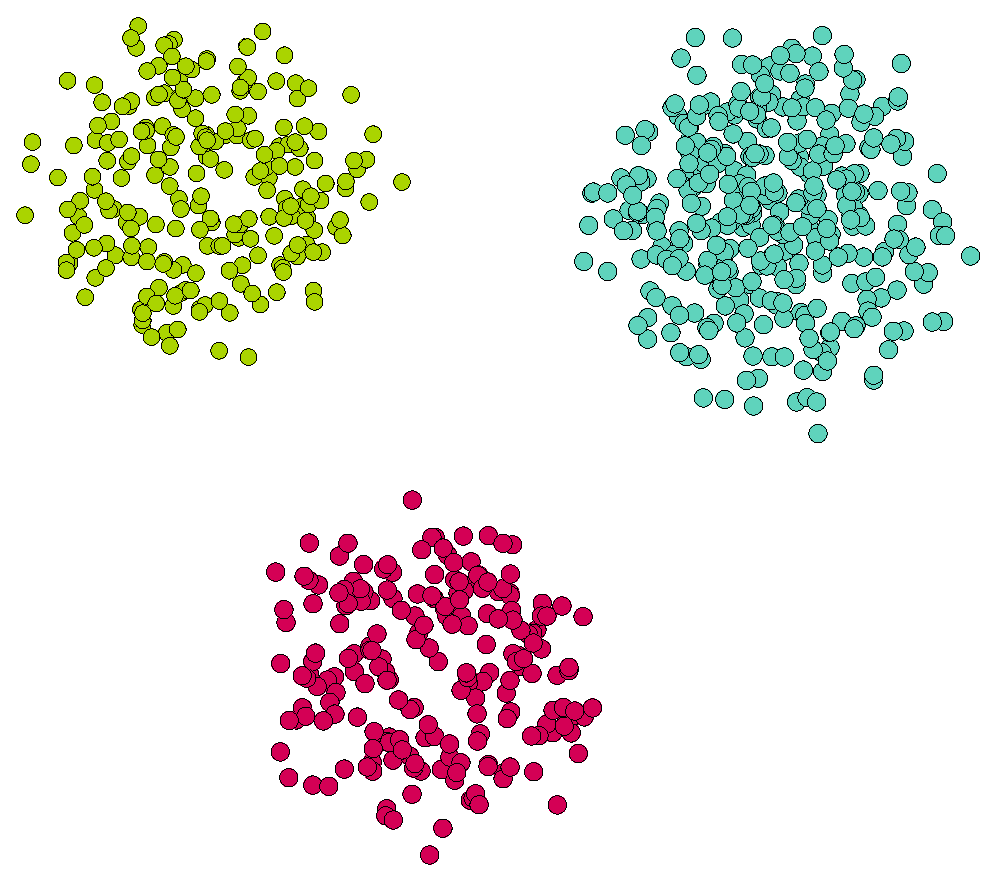
\includegraphics[width=.5\linewidth]{img/wellSeparatedObjects.eps}
  \caption{Well sepatated objects}
  \label{fig:wellSeparatedObjects}
\end{subfigure}
\begin{subfigure}{.49\textwidth}
  \centering
  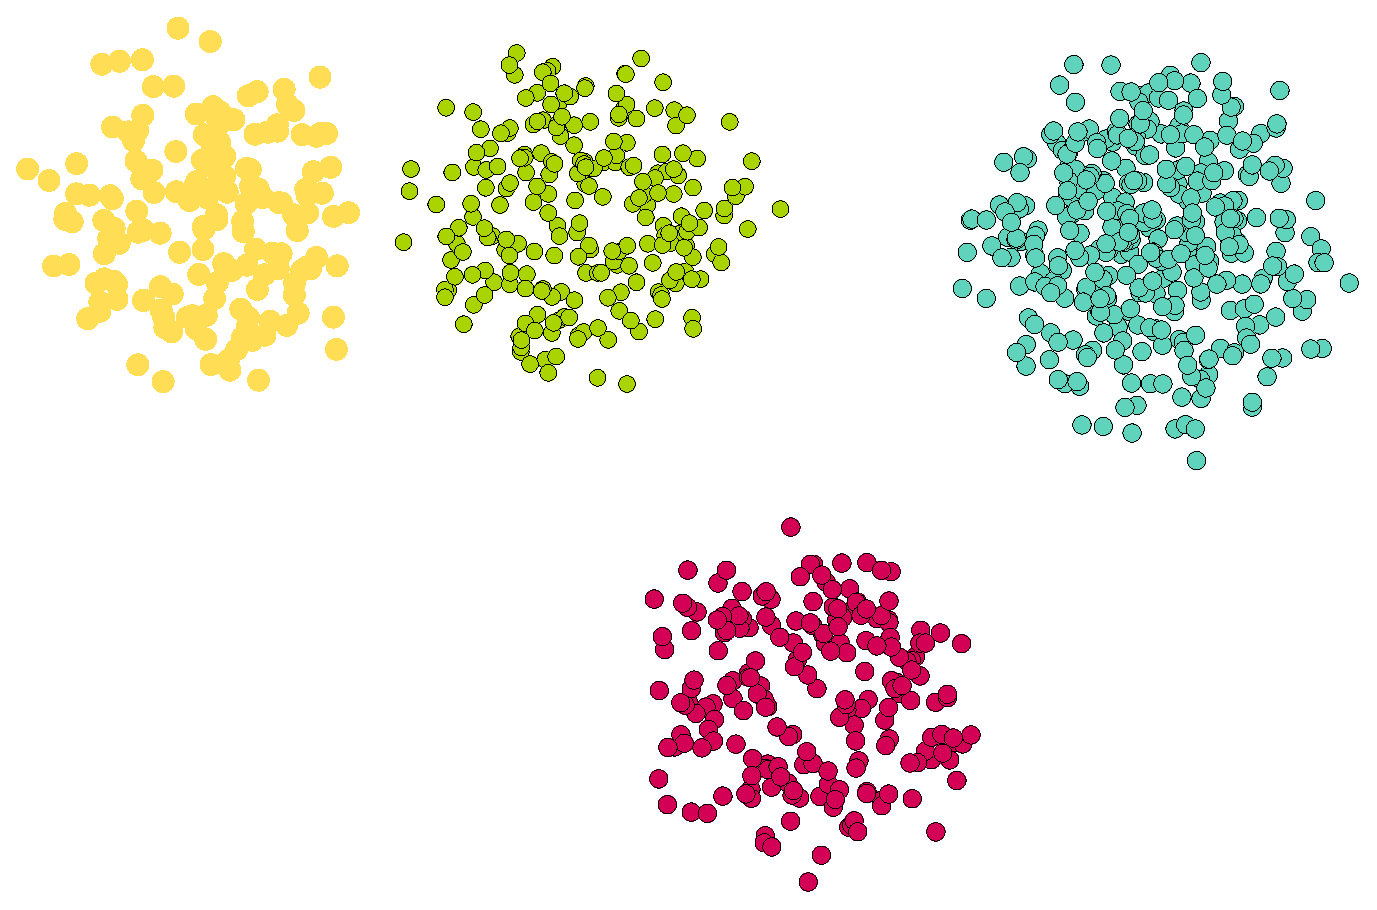
\includegraphics[width=.5\linewidth]{img/centerBasedClusters.eps}
  \caption{Center-Based Clusters}
  \label{fig:centerBasedClusters}
\end{subfigure}
\vspace*{0.5cm} 
\begin{subfigure}{.49\textwidth}
  \centering
  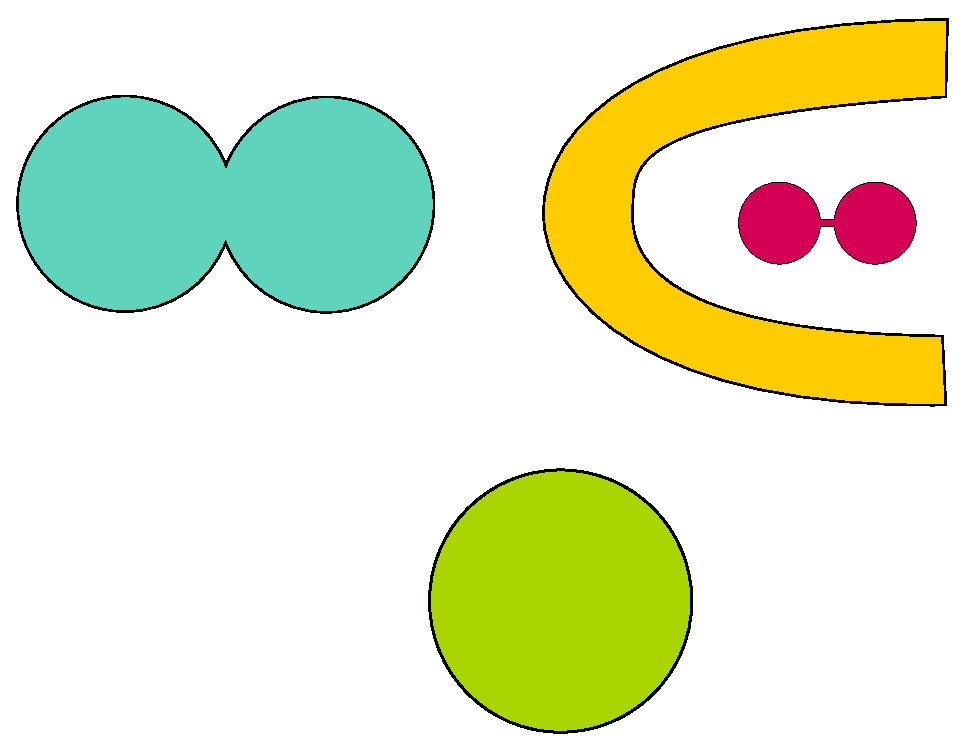
\includegraphics[width=.5\linewidth]{img/contiguousClusters.eps}
  \caption{Contiguous Clusters}
  \label{fig:contiguousClusters}
\end{subfigure}
\begin{subfigure}{.49\textwidth}
  \centering
  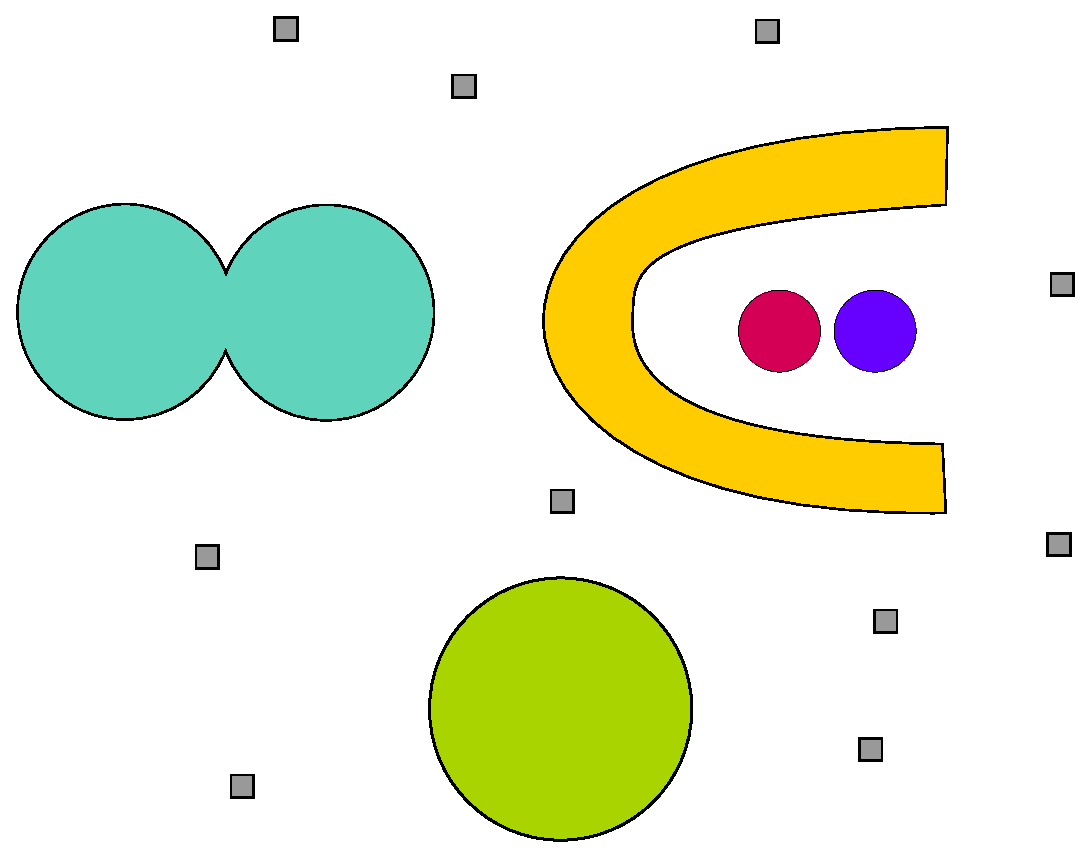
\includegraphics[width=.5\linewidth]{img/densityClusters.eps}
  \caption{Density-Based Clusters (Gray squares represent noise)}
  \label{fig:densityClusters}
\end{subfigure}
\vspace*{0.5cm} 
\begin{subfigure}{.49\textwidth}
  \centering
  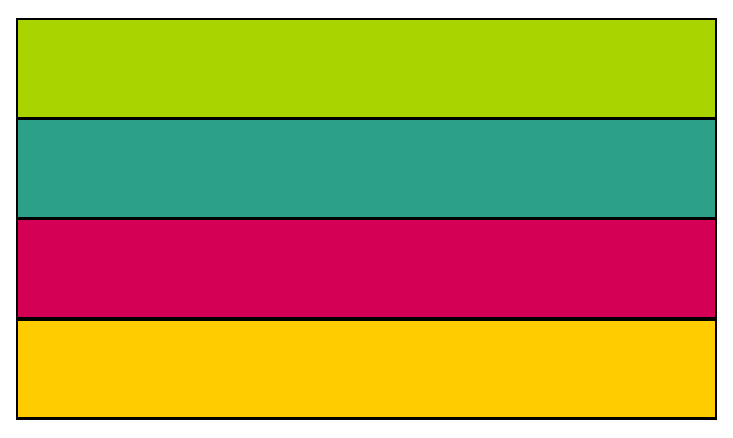
\includegraphics[width=.5\linewidth]{img/conceptualClusters.eps}
  \caption{Conceptual Clusters (Points in cluster have y-coordinate from specific range, omitting x-coordinate)}
  \label{fig:conceptualClusters}
\end{subfigure}
\begin{subfigure}{.49\textwidth}
  \centering
  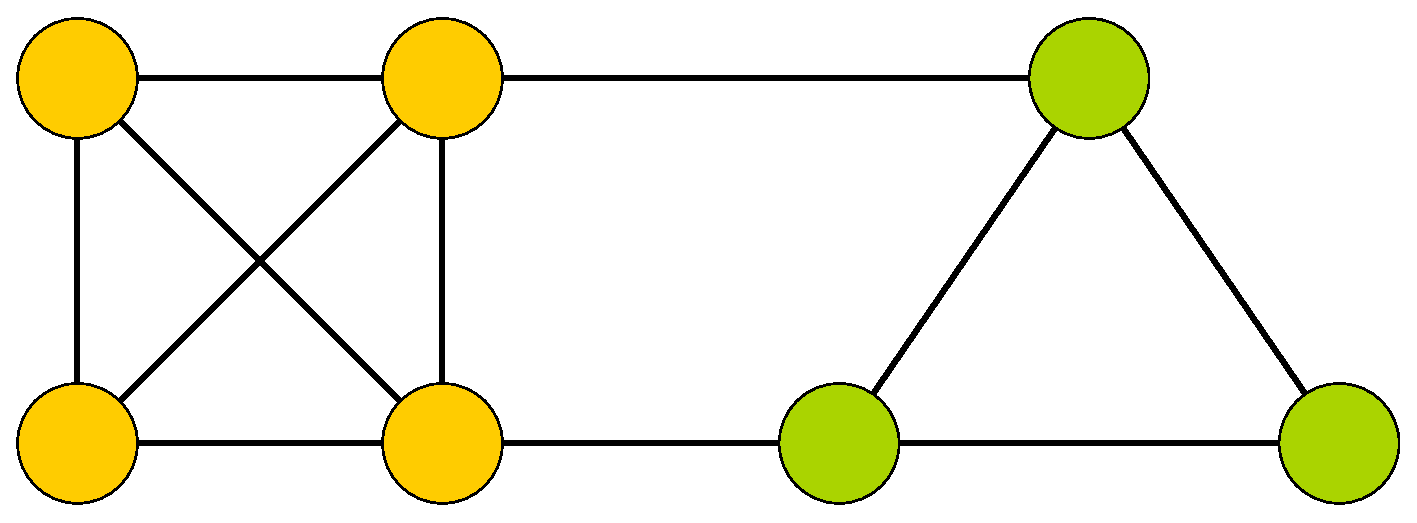
\includegraphics[width=.5\linewidth]{img/graphClusters.eps}
  \caption{Graph-Based Clusters}
  \label{fig:graphClusters}
\end{subfigure}
\caption{Typical cluster models}
\end{figure}

\begin{description}
\item[Well-Separated Clusters] Objects are easily separable-chunks of objects are not overlapping and split by sparse or empty area. Cluster is a set of objects such that each object in cluster is closer to objects from its cluster than to objects from other clusters~\autoref{fig:wellSeparatedObjects}. This is the easiest data input and most of algorithms performs well in this case.

\item[Center-Based Clusters] Object belongs to cluster if it is closer to the ``center'' of the cluster than ``centers'' of all other clusters.~\autoref{fig:centerBasedClusters} Center of cluster is usually called centroid or mean and it could represents whole cluster. This is good model for algorithms based on distance between object and centroid. \\
The best algorithm for solving this task is \textit{\textbf{Center-based clustering}} representing clusters as central object, which may not be part of the input data set.  For example \textit{\textbf{k-means}} algorithm takes $k$ centers and than each object is assigned to nearest center. Again, many metrics could be used, but commonly \textit{Euclidian distance} or \textit{Squared Euclidian distance} is used. \textit{\textbf{k-means}} clustering is basically an optimization problem where we looking for $k$ centers so distances will be the lowest possible. Problem is that optimization itself is NP-hard problem, so solution is commonly only approximate solution is searched. Approximation is commonly done by many iterations consist of assigning clusters to objects and  counting new means.
There are many variants of \textit{\textbf{k-means}} algorithm which will be described later. %TODO add ref too kmeans section

One of the biggest problems of \textit{\textbf{k-means}} algorithms is that the number of clusters must be specified at the beginning. Second problem is that clusters with similar size are used (in term of distance, not number of contained objects). This usually leads to splitting bigger clusters into smaller ones, because algorithm optimize cluster centers, not borders.
Output of \textit{\textbf{k-means}} like algorithms is usually input data set split in \textit{Voronoi cells} which could be useful for some problems.

\item[Contiguous Clusters] This model is similar to Center-Based Clusters model but there is difference that two clusters can merge into one. In other words, object is in cluster if it is similar to one ore more other objects from cluster.~\autoref{fig:contiguousClusters}\\
Main idea of \textbf{Contiguity-based clustering} is that objects that are nearby are more related than objects that are farther, so these algorithms grouping objects based on their distance only. Each cluster can be described by sum of distances or by maximum distance needed to connect objects in cluster. Having these cluster property, they can be easily ordered into hierarchy so parent clusters needs little more distance to connect its objects. This hierarchy could be represented as a dendrogram, which is tree diagram showing cluster hierarchy.\\

Other problem is the selection of linkage criterion, because cluster consists of many objects, there are many choices to compute the distance to. There are several methods for choosing linkage criteria between two sets of objects $A$ and $B$, $d$ is chosen metric:
\begin{description}
\item[Maximum or complete linkage clustering] $$\max\{d(a,b) : a \in A, b \in B\}$$
\item[Minimum or single linkage clustering] $$\min\{d(a,b) : a \in A, b \in B\}$$
\item[Mean or average linkage clustering, or UPGMA] (Unweighted Pair Group Method with Arithmetic Mean) $$\frac{1}{|A||B|}\sum_{a \in A} \sum_{b \in B} d(a,b)$$
\item[Centroid linkage clustering, or UPGMC] (Unweighted Pair-Group Method using Centroids) $$\|c_a - c_b\| \mbox{ where } c_a \mbox{ and } c_b \mbox{ are the centroids of clusters } A \mbox{ and } B$$
\item[Minimum energy clustering] $$\frac{2}{nm}\sum_{i,j=1}^{n,m}\|a_i-b_j\|_2-\frac{1}{n^2}\sum_{i,j=1}^{n}\|a_i-a_j\|_2-\frac{1}{m^2}\sum_{i,j=1}^{m}\|b_{i}-b_{j}\|_{2}$$
\end{description}

These methods are not resistive for extreme objects, which cause generating new clusters or even merging others. Methods has generally $O(n^3)$ complexity so they are slow for large amount of data. There exist optimization for special cases which has only complexity $O(n^2)$. These methods are taken as obsolete.

\item[Density-Based Clusters] Clusters are dense regions of objects. They are separated by low-density regions. This method is useful when some noise is present because the low-density regions will cover them and clusters will not change.~\autoref{fig:densityClusters} \\
Clusters in \textbf{Density-based clustering} are defined as areas with higher density of objects than in the rest of input data. Standalone objects are taken as noise. One of the most popular method is \textit{DBSCAN}. It is similar to contiguity-based clustering, because it connecting points based on the distance, but it only connects points satisfying density criterion. This means that in neighborhood specified by distance must be a minimum number of objects. These objects are called core objects and form the basis of cluster. Than objects which do not satisfy the density criterion but are close enough to at least one point from the cluster are added to cluster too.\\
The advantage of this method is its computational modesty, because it require only linear number of range queries. This method is deterministic so there is no need to tun it in iterations.
Drawback of these methods is the $\epsilon$ density parameter so borders of clusters with smaller density could be interpreted as  noise. Also separating nearby clusters may cause problems to these methods.

\item[Distribution models] Clusters in distribution models are objects that belong to same probability distribution. It is possible that one object belongs to more clusters.\\
In \textbf{Distribution-based clustering}, clusters are defined as objects from the same or similar distribution. This approach basically emulates process of generating the input data and try to reconstruct the lost statistical parameters. Main problem of this typ of clustering is problem known as \textit{overfitting}. This means that more complex model is described by less complex one and the difference between them is marked as deviation or noise. For example 3 points from the neighborhood of parabola vertex will be described by linear function.\\
One of methods used in distribution-based clustering is \textit{Gaussian mixture models} where algorithm iteratively optimizing parameters of fixed number of Gaussian distributions.
Problem is that this method assuming Gaussian distributed data set, but this set may not have even a model.

\item[Conceptual Clusters] Objects in cluster has some properties same or similar, but other properties could differ significantly.~\autoref{fig:conceptualClusters}\\
As algorithm for Conceptual Clusters, we can use algorithm depends on other model properties and less significant properties of objects could be easily omitted.

\item[Graph-Based Models] For example cliques in graphs should represent clusters. Clique is subset of nodes where every two nodes are connected with edge.~\autoref{fig:graphClusters}\\
Because of special demands of this model, special algorithms are needed so we could use graph algorithms, for example Bron-Kerbosch algorithm for finding cliques. %TODO source!
\end{description}

Based on cluster organization~\ref{sec:clusterorganization} there is also another option for splitting clustering algorithms by type of objects relationship. Not all types could be used by each cluster model.

\begin{description}
\item[Strict partitioning clustering] Objects belongs exactly into one cluster.
\item[Strict partitioning clustering with outliers] Simillar to \textit{\textbf{strict partitioning clustering}} but isolated objects can be also unassigned. 
\item[Overlapping clustering] Object may belong to multiple clusters and we can specify, how much object belong to each cluster for example in percent.
\item[Hierarchical clustering] Object belongs also into parent clusters.
\end{description}

 Because calculation with no strictly assigned objects is to complex and does not bring many advantages, in this thesis we have focused on strict clustering only.\\
 
 Clustering algorithms are wide class of algorithms so we could not focused one every clustering model and appropriate algorithm and speed it up by parallelization, because there does not exist any universal approach for speeding up but on the contrary it needs to use every single detail of the algorithm. We want to choose one of the most versatile algorithm so we decided for k-means algorithm for its wide range of usage and undemanding on the properties of the input data.\\
K-means algorithm~\cite{hartigan1979algorithm}, which input is set of $n$ points in $d$-dimensional space $R^d$ a number of output clusters $k$ and a number of maximum iterations $i$. The task is to assign points to centroids (centers of clusters) and minimize the distance between points assigned to one cluster and appropriate centroid. Algorithm works iteratively and each iteration consist of two steps. At first step points are assigned to the nearest centroids and than in the second step, new centroids are computed as a mean of all points assigned to each cluster. Algorithm ends after known number of steps or when nothing changes between two iterations. Output of the this algorithm are centroids coordinates or points with assigned clusters.
Because k-means is universal algorithm, there exists some variants if classical k-means algorithm is inconvenient or unusable.
There also exist few variations:
\begin{description}
\item[k-medoids] - centroids are not virtual points in $R^d$ space but point from input data whose average dissimilarity to all other objects in cluster is minimal. This variant is useful when non-existing mean is unusable.
\item[k-medians] - same algorithm as k-means, but median is used instead of mean for computing new centroid.
\item[k-means++] - initial centers are chosen randomly. This selection avoid bad inputs.
\item[Fuzzy C-means] - fuzzy cluster~\ref{sec:clusterorganization} assignment is allowed. Object does not belong strictly to one centroid but it has degree of belonging to cluster.
\end{description}

Disadvantages of k-means algorithm is that we need to know the number of output clusters at the beginning and after computation start this number could not be changed. This possibility might be demanded by some type of problems and k-means is inconvenient for them.\\
Also size of clusters could be problem in some cases because the main goal of k-means is to minimize the distance inside the cluster, we could have input data where one cluster contains many objects and one smaller cluster with only a few objects~\autoref{fig:kmeansbadinput}. Than k-means divide the bigger cluster~\autoref{fig:kmeansbadoutput} so some objects from bigger that are closer centroid to smaller cluster are assigned to smaller cluster which could be undesirable because k-means ignores input data distribution.

\begin{figure}[h]
\centering
\begin{subfigure}{.49\textwidth}
  \centering
  \includegraphics[width=.5\linewidth]{img/kmeans_badsample1.eps}
  \caption{Input data (assigned to clusters only for demonstration)}
  \label{fig:kmeansbadinput}
\end{subfigure}
\begin{subfigure}{.49\textwidth}
  \centering
  \includegraphics[width=.5\linewidth]{img/kmeans_badsample2.eps}
  \caption{k-means output}
  \label{fig:kmeansbadoutput}
\end{subfigure}
\caption{CPU and GPU architecture comparison}
\end{figure}

\begin{Code}
    \centering
\begin{lstlisting}[caption={k-means algorithm}, language=C++, escapeinside={\%*}{*)}, label={lst:kMeansCode}, numbers=left]
// Assign points to clusters
%*\label{lst:assignOuterForLoop}*)assign_to_clusters(data, means) {
//Iterate through data
%*\label{lst:assignInnerForLoop}*)  for( d = 0; d < data_size; d++) {
// Iterate through means
    for( m = 0; m < means_size; m++) {
      distance = count_distance( data[d], means[m] );
// If m-cluster is closer, reassign cluster
      if ( distance < min_distance ) {
        assigned_cluster = m;
        min_distance = distance;
      }
    }
    data[d]->assigned_cluster = assigned_cluster;
  }
}
\end{lstlisting}
    \caption{Code for first step - assigning points to clusters}
\end{Code}

If we look closer to k-means algorithm and decompose the first step, we realize that it consist of two nested  loops. First loop~\autoref{lst:assignOuterForLoop} iterates through all objects and than the second one iterates through centroid and looking to nearest one. Parallelization of the first loop is not a problem because we could run a separate thread for each object and determine the nearest centroid, because there are no race conditions. Parallelization of the second loop~\autoref{lst:assignInnerForLoop} is little bit harder but when we have parallel version of minimum function, we are done too.\\

\begin{Code}
    \centering
\begin{lstlisting}[caption={k-means algorithm}, language=C++, escapeinside={\%*}{*)}, label={lst:kMeansCode}, numbers=left]
// Compute new means
%*\label{lst:computeNewMeans}*)compute_means(data, means) {
// Iterate through data and accumulate data in appropriate new mean
  for( d = 0; d < data_size; d++) {
    assigned_cluster = data[d]->assigned_cluster;
    new_means[assigned_cluster]->contained_points++;
    new_means[assigned_cluster]->coordinates +=
      data[d]->coordinates;
  }
  
// Count new means coordinates (arithmetic mean)
  for( m = 0; m < means_size; m++) {
    new_means[m]->coordinates /=
      new_means[m]->contained_points;
  }
}
\end{lstlisting}
    \caption{Code for second step - computing new means}
\end{Code}
Parallelizing of the second step of the algorithm is harder because there are compute dependencies. We need to compute new centroids which contains to accumulate object assigned to same cluster, This is problem because we could not run thread per each point - accumulating objects could be accessed from different threads and will probably cause corruption of result.
One possibility is to swap loops and parallelize loop iterating through clusters and avoid described collision because each thread compute one new mean and computation could not be break by another thread. Problem is that parallelization of the object loop ii much bigger and parallelizing it could speed up the computation much more. This could be solved by accumulating objects in thread local variable but than these partial results must be merged into a single one which takes some extra time.
If we parallelize the bigger loop in second step we could merge both steps into single one and accumulate newly assigned objects into thread local variables and get some more speed improvement.